\chapter{Réalisation et implémentation}

Après avoir présenté l'analyse des besoins et la conception du système, ce chapitre est consacré à la phase de réalisation et d'implémentation de notre application de gestion des consultations médicales. Il a pour objectif de présenter les choix techniques adoptés, l'environnement de développement utilisé ainsi que les différentes étapes de mise en œuvre de la solution.

Nous commencerons par présenter les outils et les technologies utilisés pour le développement de l'application, avant de décrire l'organisation de sa structure et la configuration de la connexion à la base de données. Nous détaillerons ensuite l'implémentation des différentes couches de l'application, notamment la couche DAO, la couche Service (si applicable), les Servlets et les pages JSP, en mettant en évidence leur rôle dans le fonctionnement du système.

Enfin, nous présenterons les principales fonctionnalités développées à travers des captures d'écran de l'application, afin d'illustrer concrètement le résultat obtenu.

\section{Environnement de développement}
La réalisation de notre application de gestion des consultations médicales a nécessité l'utilisation de plusieurs outils permettant de développer, exécuter et gérer l'application dans de bonnes conditions. Ces outils ont été choisis en fonction des besoins du projet et de l'architecture adoptée, basée sur le modèle \textbf{MVC}.

L'environnement de développement repose principalement sur\textbf{ IntelliJ IDEA} pour l'écriture et la gestion du code source, \textbf{Apache Tomcat} pour le déploiement et l'exécution de l'application web, ainsi que \textbf{DBeaver} pour la gestion et l'exécution de la base de données.

Les principaux outils utilisés sont présentés ci-dessous.

\subsection{IntelliJ IDEA}
IntelliJ IDEA est l'environnement de développement intégré (IDE) utilisé pour la réalisation de notre application. Il permet d'écrire, d'organiser et de déboguer le code Java, ainsi que de gérer les différentes composantes du projet, notamment les Servlets, les classes DAO, les services et les pages JSP.
\begin{figure}[h!]
\centering

\includegraphics[width=0.4\textwidth]{images/intellij.png}
\caption{Environnement de développement IntelliJ IDEA}
\end{figure}
\subsection{Apache Tomcat}
Apache Tomcat est le serveur web utilisé pour déployer et exécuter notre application. Il prend en charge les technologies Servlet et JSP, permettant ainsi de traiter les requêtes HTTP envoyées par les utilisateurs et de générer les réponses correspondantes.

Il assure notamment la communication entre les différentes composantes de l'application web et le navigateur de l'utilisateur.
\begin{figure}[h!]
	\centering
	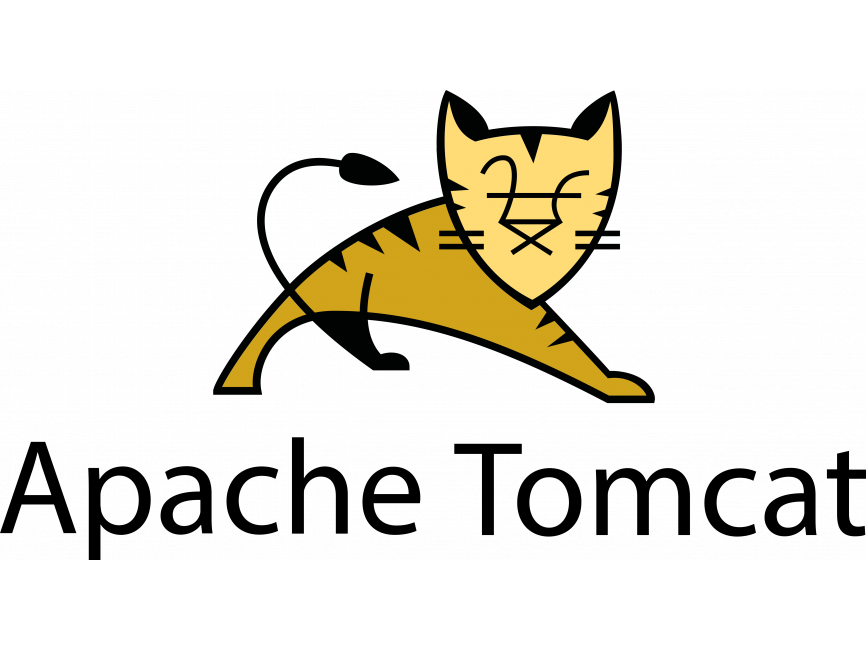
\includegraphics[width=0.5\textwidth]{images/apacheTomcat.png}
	\caption{Serveur Apache Tomcat}
\end{figure}
\newpage
\subsection{DBeaver}
DBeaver est un outil de gestion de bases de données utilisé pour accéder à la base MySQL et interagir avec ses différentes tables. Il permet notamment d'exécuter des requêtes SQL, de consulter les données enregistrées et de vérifier les opérations effectuées par l'application.
\begin{figure}[h!]
	\centering
	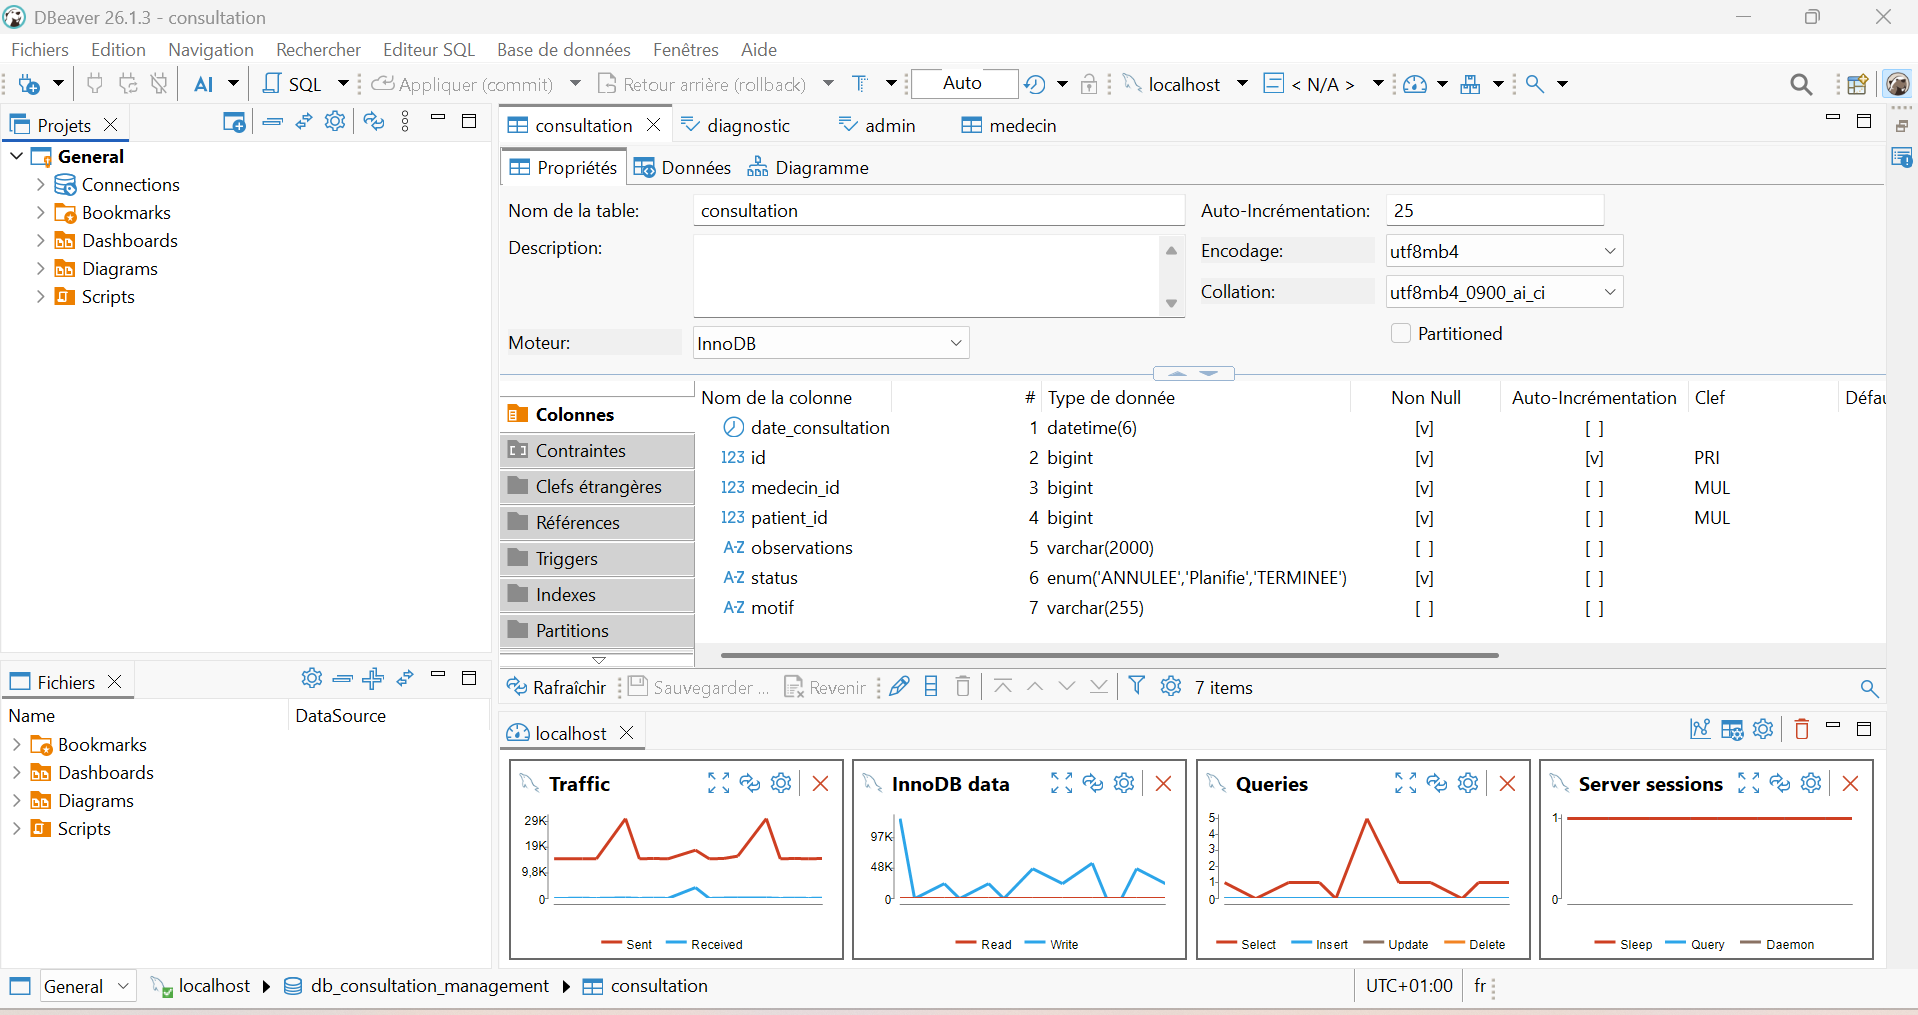
\includegraphics[width=\textwidth]{images/dbeaver.png}
	\caption{Interface de gestion de base de données DBeaver}
\end{figure}

\subsection{Draw.io}
Draw.io est un outil de création de diagrammes utilisé lors des phases d'analyse et de conception du projet. Il permet de représenter graphiquement les différents éléments du système à travers des diagrammes UML et des modèles de données.

Dans le cadre de notre projet, cet outil a été utilisé pour réaliser les différents diagrammes nécessaires à la modélisation de l'application, notamment les diagrammes de cas d'utilisation, de classes et d'états de transition.
\begin{figure}[h!]
	\centering
	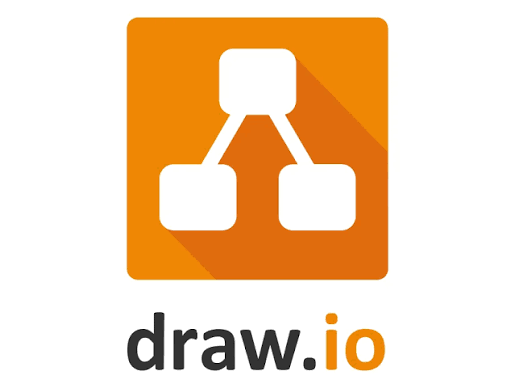
\includegraphics[width=0.4\textwidth]{images/drawio.png}
	\caption{Drawio}
\end{figure}
\subsection{Git et GitHub}
Git est un système de gestion de versions permettant de suivre les modifications apportées au code source tout au long du développement. Il facilite la gestion des différentes versions du projet et permet de revenir à un état précédent en cas de besoin.

GitHub est une plateforme d'hébergement de dépôts Git qui facilite le travail collaboratif entre les membres de l'équipe. Dans le cadre de notre projet, il a été utilisé pour centraliser le code source, partager les modifications et assurer le suivi de l'évolution de l'application.
\begin{figure}[h!]
	\centering
	
\includegraphics[width=0.4\textwidth]{images/git.png}
	
\includegraphics[width=0.4\textwidth]{images/github.png}
	\caption{Git Github}
\end{figure}

\section{Technologies utilisées}
Le développement de notre application de gestion des consultations médicales repose sur plusieurs technologies permettant d'assurer le fonctionnement de ses différentes composantes. Le choix de ces technologies répond aux besoins d'une application web dynamique, organisée selon l'architecture MVC et reposant sur une base de données relationnelle.

Les principales technologies utilisées sont présentées ci-dessous.
\subsection{Java 21}
Java 21 est le langage de programmation utilisé pour développer la partie serveur de notre application. Il permet d'implémenter la logique métier ainsi que les différentes composantes nécessaires au fonctionnement du système, notamment les classes DAO, les services et les Servlets.
\begin{figure}[h!]
	\centering
	
\includegraphics[width=0.5\textwidth]{images/JDK.jpeg}
	\caption{}
\end{figure}
\subsection{Jakarta EE}
Jakarta EE constitue l'ensemble de spécifications utilisé pour le développement de la partie serveur de notre application web. Nous nous sommes principalement appuyés sur les technologies Servlet et JSP pour gérer les requêtes des utilisateurs et générer les interfaces dynamiques.
\subsection{JSP et Servlets}
Les JSP (JavaServer Pages) et les Servlets sont utilisées pour assurer la communication entre l'utilisateur et la partie serveur de l'application.
\begin{itemize}
	\item \textbf{Servlets :} elles assurent le traitement des requêtes HTTP, la récupération des données envoyées par les utilisateurs et la coordination avec les couches DAO et Service.
	\item \textbf{JSP :} elles permettent de générer les interfaces dynamiques affichées dans le navigateur, en présentant les informations récupérées depuis la partie serveur.
\end{itemize}
\subsection{JDBC}
JDBC (Java Database Connectivity) est une API Java permettant d'établir la communication entre l'application et la base de données MySQL.

Elle est utilisée pour exécuter les requêtes SQL nécessaires aux opérations de manipulation des données, notamment l'insertion, la consultation, la modification et la suppression des enregistrements.


\subsection{Hibernate }
Hibernate est un framework de persistance Java basé sur le principe du mapping objet-relationnel (ORM). Il permet de faire correspondre les classes Java aux tables de la base de données relationnelle et de manipuler les données à travers des objets Java.

Dans notre application, Hibernate est utilisé pour faciliter les interactions avec la base de données MySQL, notamment lors des opérations de persistance, de récupération, de modification et de suppression des données. Il permet ainsi de réduire la quantité de code SQL nécessaire à la manipulation des entités.

\subsection{MySQL}
MySQL est le système de gestion de base de données relationnelle utilisé pour stocker et organiser les informations de l'application.

Il permet de gérer les différentes données liées au système, notamment les informations des patients, des médecins et des consultations, tout en assurant les relations entre les différentes tables.

\subsection{HTML, CSS, Bootstrap et JavaScript}
Pour la réalisation des interfaces utilisateur, nous avons utilisé plusieurs technologies front-end :
\begin{itemize}
\item \textbf{ HTML }: permet de structurer le contenu des différentes pages de l'application.
\item \textbf{CSS} : permet de définir la présentation visuelle et la mise en forme des interfaces.
\item \textbf{Bootstrap} : facilite la création d'interfaces responsives grâce à ses composants et ses classes prédéfinies.
\item \textbf{JavaScript} : utilisé pour ajouter quelques interactions et comportements dynamiques du côté client.
\end{itemize}
\subsection{Apache Maven}
Apache Maven est un outil de gestion et d'automatisation de projets Java. Il permet de gérer les dépendances du projet, de faciliter leur téléchargement et leur intégration, ainsi que d'organiser le processus de compilation et de construction de l'application.

Dans notre projet, Maven est utilisé pour gérer les bibliothèques nécessaires au fonctionnement de l'application, notamment celles liées à Jakarta EE, JDBC et Hibernate. La configuration des dépendances et des paramètres du projet est centralisée dans le fichier pom.xml.
\begin{figure}[h!]
	\centering
	
\includegraphics[width=0.4\textwidth]{images/maven.jpeg}
	\caption{Apache Maven}
\end{figure}

\section{Structure du projet}
L'application a été développée en suivant le modèle architectural MVC (Model-View-Controller), enrichi par une séparation en couches DAO et Service. Cette organisation permet de séparer les responsabilités de chaque composante et de faciliter la maintenance et l'évolution du projet.

La structure générale repose sur les éléments suivants :
\begin{itemize}
\item \textbf{Model }: regroupe les classes représentant les entités métier et les données manipulées par l'application.
\item \textbf{DAO (Data Access Object)} : assure les interactions avec la base de données à travers JDBC. Cette couche regroupe les opérations de lecture et de manipulation des données.
\item \textbf{Service :} contient la logique métier de l'application et assure la coordination entre les Servlets et les DAO.
\item \textbf{Controller :} représenté par les Servlets, il reçoit les requêtes HTTP, fait appel aux services appropriés et transmet les résultats aux vues.
\item \textbf{View :} composée des pages JSP, elle assure l'affichage des données et l'interaction avec l'utilisateur.
\end{itemize}
Cette séparation permet de limiter le couplage entre les différentes parties de l'application et de rendre le code plus organisé.

\begin{figure}[h!]
	\centering
	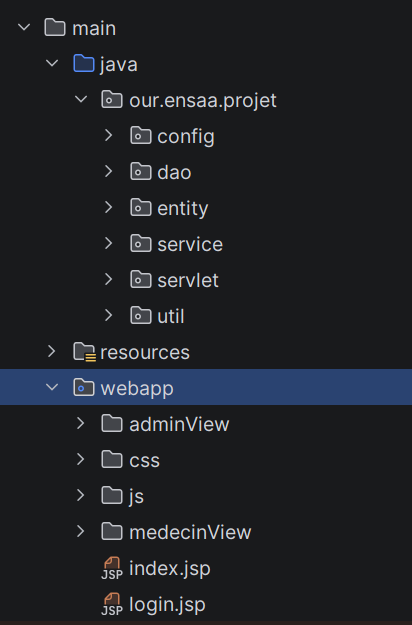
\includegraphics[width=0.6\textwidth]{images/structure.png}
	\caption{Organisation générale de la structure du projet}
\end{figure}
\section{Configuration de la connexion à la base de données}
La connexion à la base de données constitue une étape essentielle dans la réalisation de notre application. Elle permet aux différentes composantes de la partie serveur d'accéder aux informations stockées dans MySQL.

Pour assurer cette communication, nous avons utilisé Hibernate comme framework ORM, associé à JDBC pour la communication avec le système de gestion de base de données MySQL.

Hibernate assure le mapping entre les objets Java et les tables relationnelles, facilitant ainsi les opérations de persistance et de manipulation des données. Sa configuration nécessite notamment la définition des paramètres de connexion, tels que l'URL de la base de données, le nom d'utilisateur, le mot de passe et le pilote JDBC.

Cette configuration permet à l'application d'établir une connexion avec la base de données et de réaliser les opérations nécessaires au fonctionnement du système.

\section{Implémentation de la couche DAO}
La couche DAO (Data Access Object) est chargée de gérer les interactions entre l'application et la base de données. Elle permet de regrouper les opérations d'accès aux données et de séparer ces opérations de la logique métier.

Dans notre application, cette couche repose sur JPA (Java Persistence API), avec Hibernate comme implémentation ORM. L'accès aux données est réalisé à travers l'interface EntityManager, qui permet d'exécuter des requêtes, de récupérer des entités et de gérer leur persistance.
\subsection{Organisation de la couche DAO}
La couche DAO regroupe les classes chargées d'effectuer les opérations de persistance pour les différentes entités de l'application.

Chaque classe DAO est associée à une entité métier et prend en charge les opérations de manipulation de ses données.
\begin{figure}[h!]
	\centering
	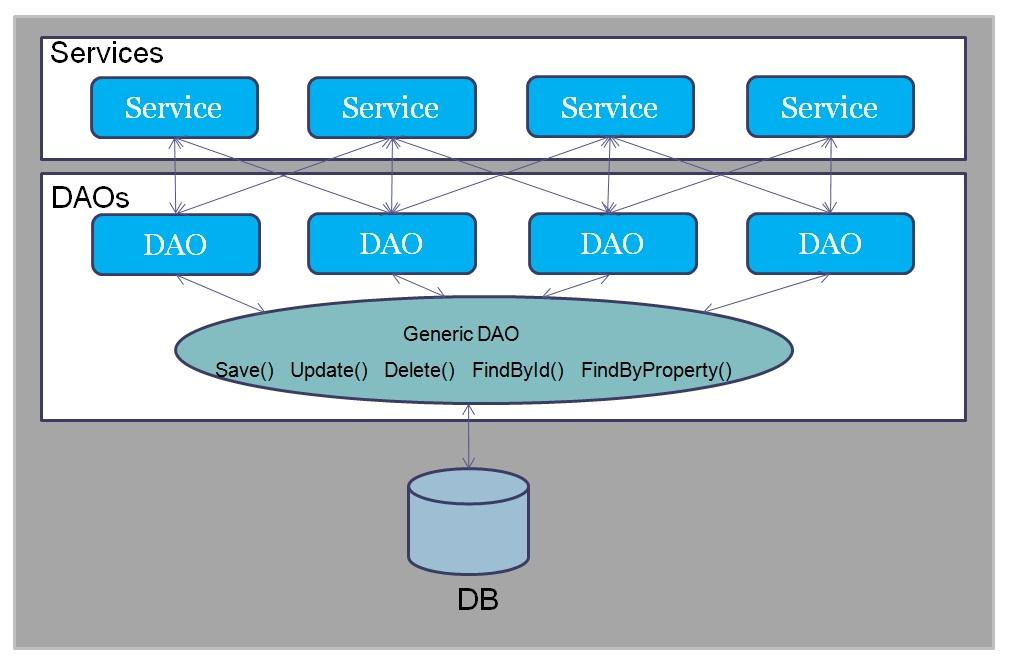
\includegraphics[width=\textwidth]{images/dao.jpg}
	\caption{Principe d'organisation de la couche DAO}
\end{figure}
\newpage
\subsection{Accès aux données avec EntityManager}
L'interface EntityManager constitue le principal mécanisme utilisé pour interagir avec les entités persistantes. Elle permet notamment d'effectuer des opérations de recherche, d'insertion, de modification et de suppression des données.

Pour récupérer des informations spécifiques, nous avons également utilisé JPQL (Java Persistence Query Language). Ce langage permet d'écrire des requêtes en se basant sur les entités Java et leurs propriétés, plutôt que directement sur les tables de la base de données.

\subsection{Exemple d'implémentation d'une méthode DAO}
Afin d'illustrer le fonctionnement de cette couche, voici un exemple extrait de notre application. La méthode getMedecinByEmail() permet de rechercher un médecin à partir de son adresse électronique.

\begin{figure}[h!]
	\centering
	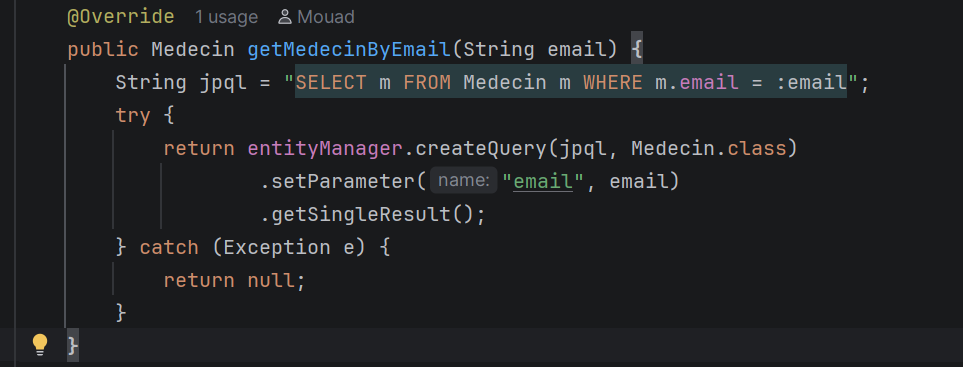
\includegraphics[width=\textwidth]{images/exemple.png}
	\caption{Implémentation de la recherche d'un médecin par email}
\end{figure}
Cette méthode utilise une requête JPQL pour rechercher un médecin dont l'adresse électronique correspond au paramètre fourni. La méthode createQuery() permet de construire une requête typée associée à l'entité Medecin, tandis que setParameter() permet de transmettre la valeur de l'adresse électronique à la requête.

Enfin, getSingleResult() permet de récupérer le résultat correspondant. En cas d'exception durant l'exécution de la requête, la méthode retourne null.

Cette approche permet de simplifier les opérations d'accès aux données tout en bénéficiant des mécanismes de mapping objet-relationnel fournis par Hibernate.

\section{Implémentation de la couche Service}

La couche Service représente la couche chargée de la logique métier de l'application. Elle se positionne entre les Servlets et les DAO afin de séparer le traitement métier des opérations d'accès aux données.

Dans notre application, elle assure la coordination des différentes opérations nécessaires à la gestion des consultations médicales. Elle permet notamment de regrouper les traitements métier et de faire appel aux méthodes appropriées de la couche DAO.

Cette organisation permet de rendre le code plus structuré, de limiter la duplication des traitements et de faciliter l'évolution de l'application.

\subsection{Rôle de la couche Service}
La couche Service intervient principalement pour :
\begin{itemize}
	\item Centraliser les traitements liés aux fonctionnalités de l'application.
	\item Faire appel aux DAO pour accéder aux données.
	\item Coordonner les différentes opérations métier.
	\item Assurer la séparation entre la logique métier et la gestion des requêtes HTTP.
\end{itemize}
\begin{figure}[h!]
	\centering
	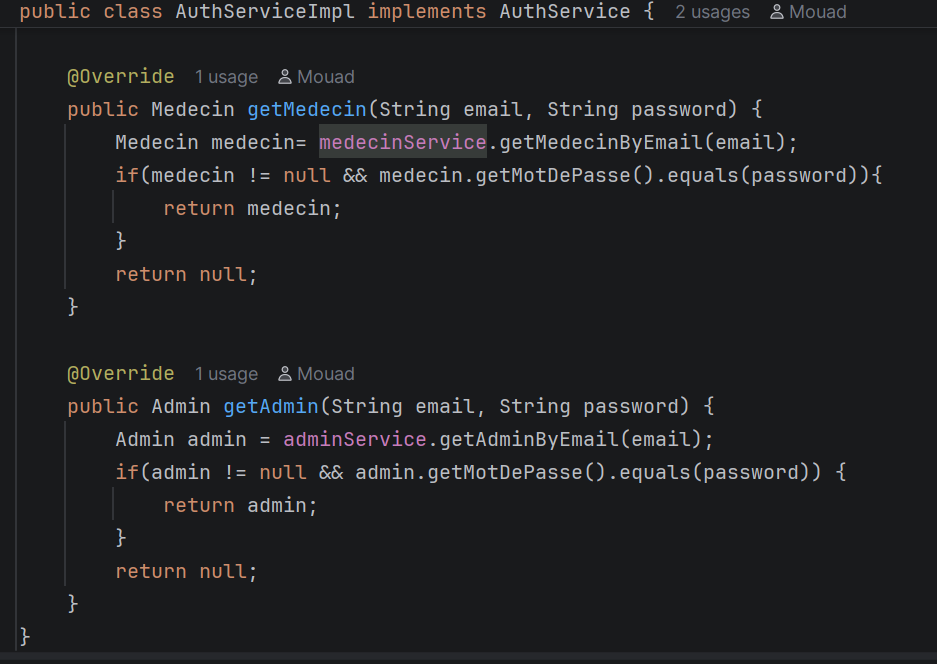
\includegraphics[width=\textwidth]{images/exempleService.png}
	\caption{Exemple d'implémentation de la couche Service}
\end{figure}

\section{Implémentation des Servlets}
Les Servlets constituent la couche de contrôle de notre application selon le modèle MVC. Elles assurent la réception et le traitement des requêtes HTTP envoyées par les utilisateurs depuis les interfaces web.

Lorsqu'un utilisateur effectue une action, la Servlet correspondante récupère les paramètres de la requête, fait appel aux méthodes nécessaires de la couche Service et prépare les données destinées à être affichées.

Elle assure ensuite la navigation vers la page JSP appropriée en transmettant les résultats du traitement.
\subsection{Traitement des requêtes HTTP}
Les Servlets utilisent principalement les méthodes suivantes :\begin{itemize}
	\item \textbf{doGet()} : permet de traiter les requêtes HTTP de type GET, notamment pour afficher des pages et récupérer des informations.
	\item \textbf{doPost() }: permet de traiter les requêtes HTTP de type POST, notamment lors de l'envoi de formulaires et de l'enregistrement de données.
\end{itemize}

\subsection{Communication avec les autres couches}
Le fonctionnement général d'une Servlet repose sur les étapes suivantes :\begin{enumerate}
	\item Réception de la requête HTTP.
	\item Récupération des paramètres transmis par l'utilisateur.
	\item Appel de la méthode correspondante dans la couche Service.
	\item Récupération du résultat du traitement.
	\item Transmission des données à la JSP à travers les attributs de la requête.
	\item Redirection ou transfert vers la vue appropriée.
\end{enumerate}

\begin{figure}[h!]
	\centering
	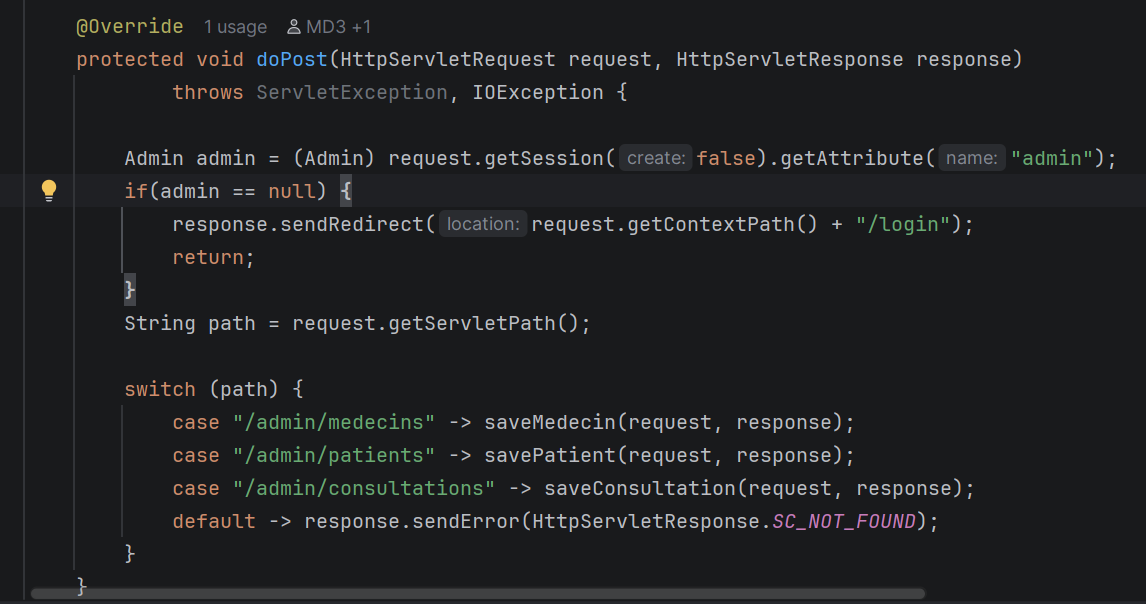
\includegraphics[width=\textwidth]{images/exempleServlet.png}
	\caption{Exemple de traitement d'une requête dans une Servlet}
\end{figure}

\section{Réalisation des interfaces JSP}
Les pages JSP constituent la couche de présentation de notre application. Elles permettent d'afficher les informations et de proposer aux utilisateurs des interfaces pour interagir avec les différentes fonctionnalités du système.

Les interfaces ont été développées à l'aide de HTML, CSS et Bootstrap, avec l'utilisation de JavaScript pour certaines interactions côté client.

Les pages JSP récupèrent les données transmises par les Servlets et les affichent sous forme de tableaux, de formulaires et d'autres composants graphiques.

\subsection{Organisation des interfaces}
Les interfaces sont organisées selon les différentes fonctionnalités de l'application. Elles permettent notamment de consulter et de gérer les informations relatives aux patients, aux médecins et aux consultations médicales.
\subsection{Présentation des interfaces réalisées}

Dans cette partie, nous présenterons les principales interfaces développées, accompagnées de captures d'écran illustrant leur fonctionnement.

\subsubsection{Page de connexion}
\begin{figure}[h!]
	\centering
	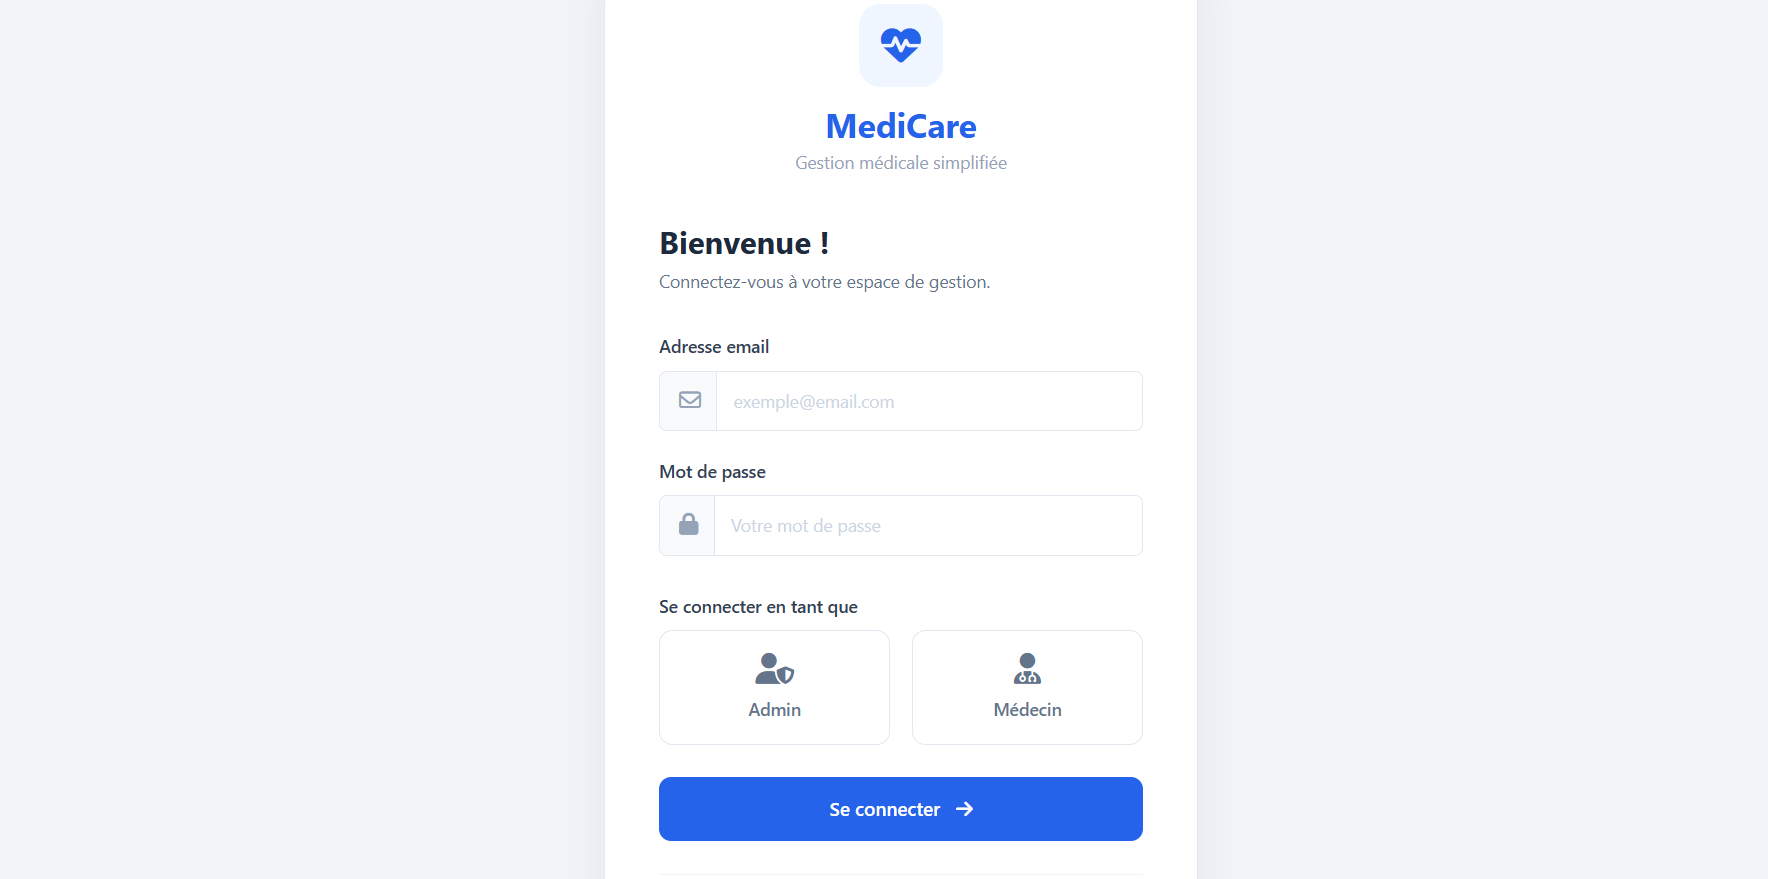
\includegraphics[width=\textwidth]{images/pageLogin.png}
	\caption{Interface permettant aux utilisateurs d'accéder à l'application.}
\end{figure}

\subsubsection{Tableau de bord}
\begin{figure}[h!]
	\centering
	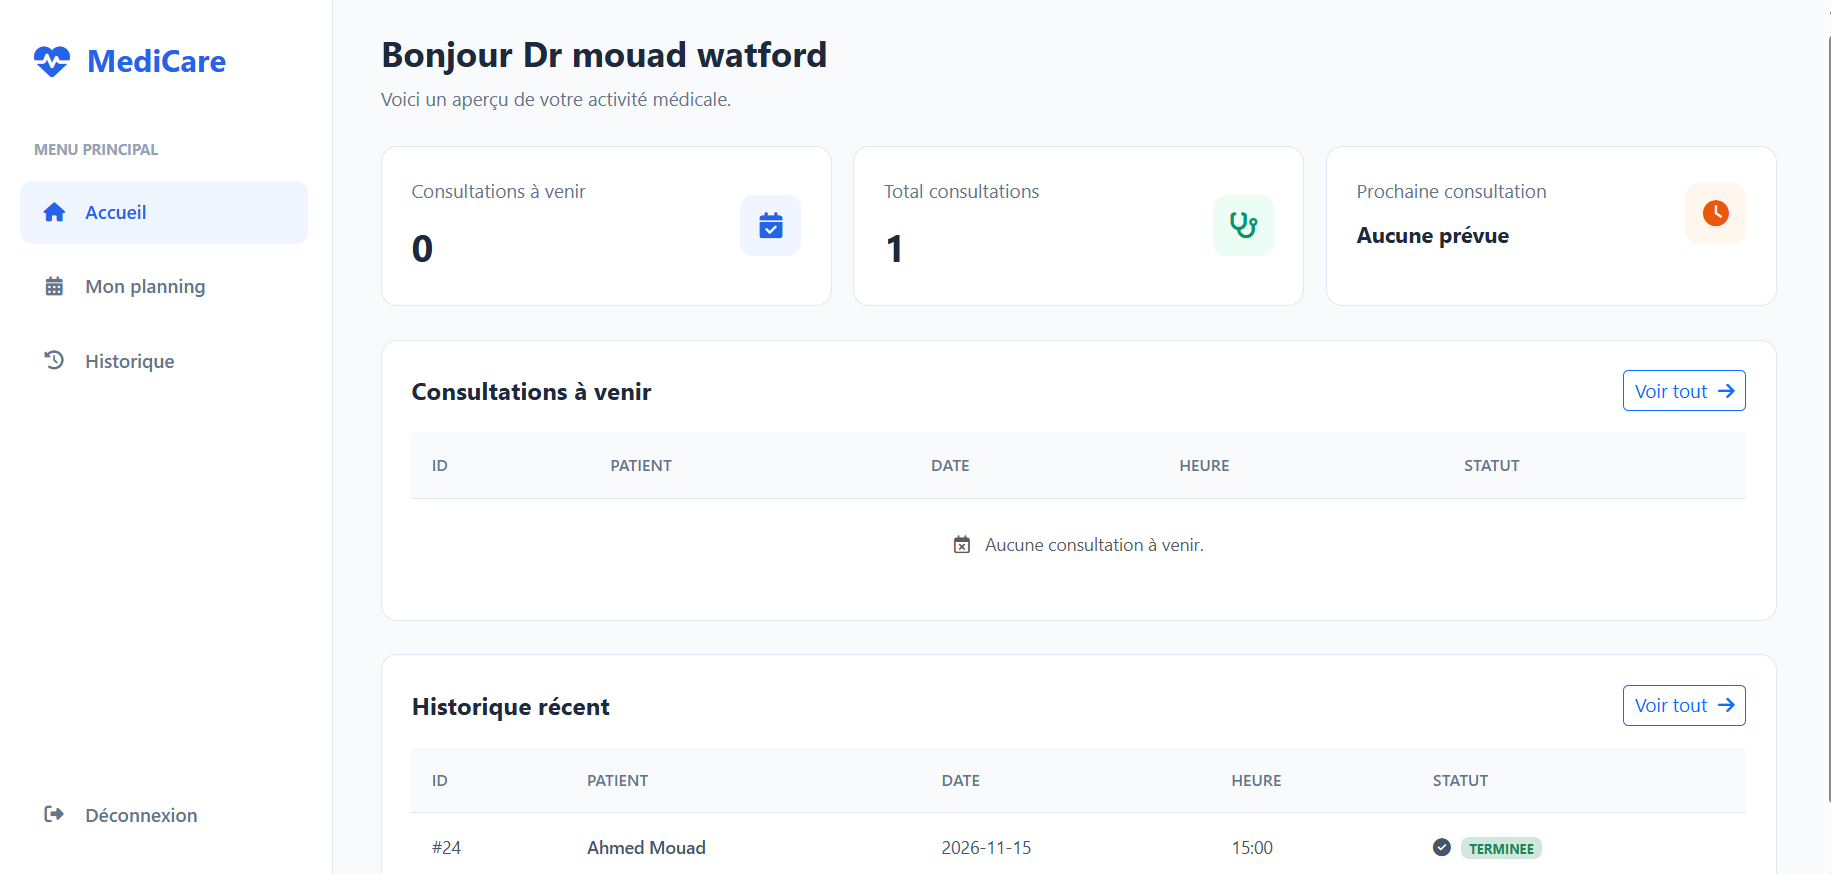
\includegraphics[width=0.4\textwidth]{images/DashboardMedecin.png}
	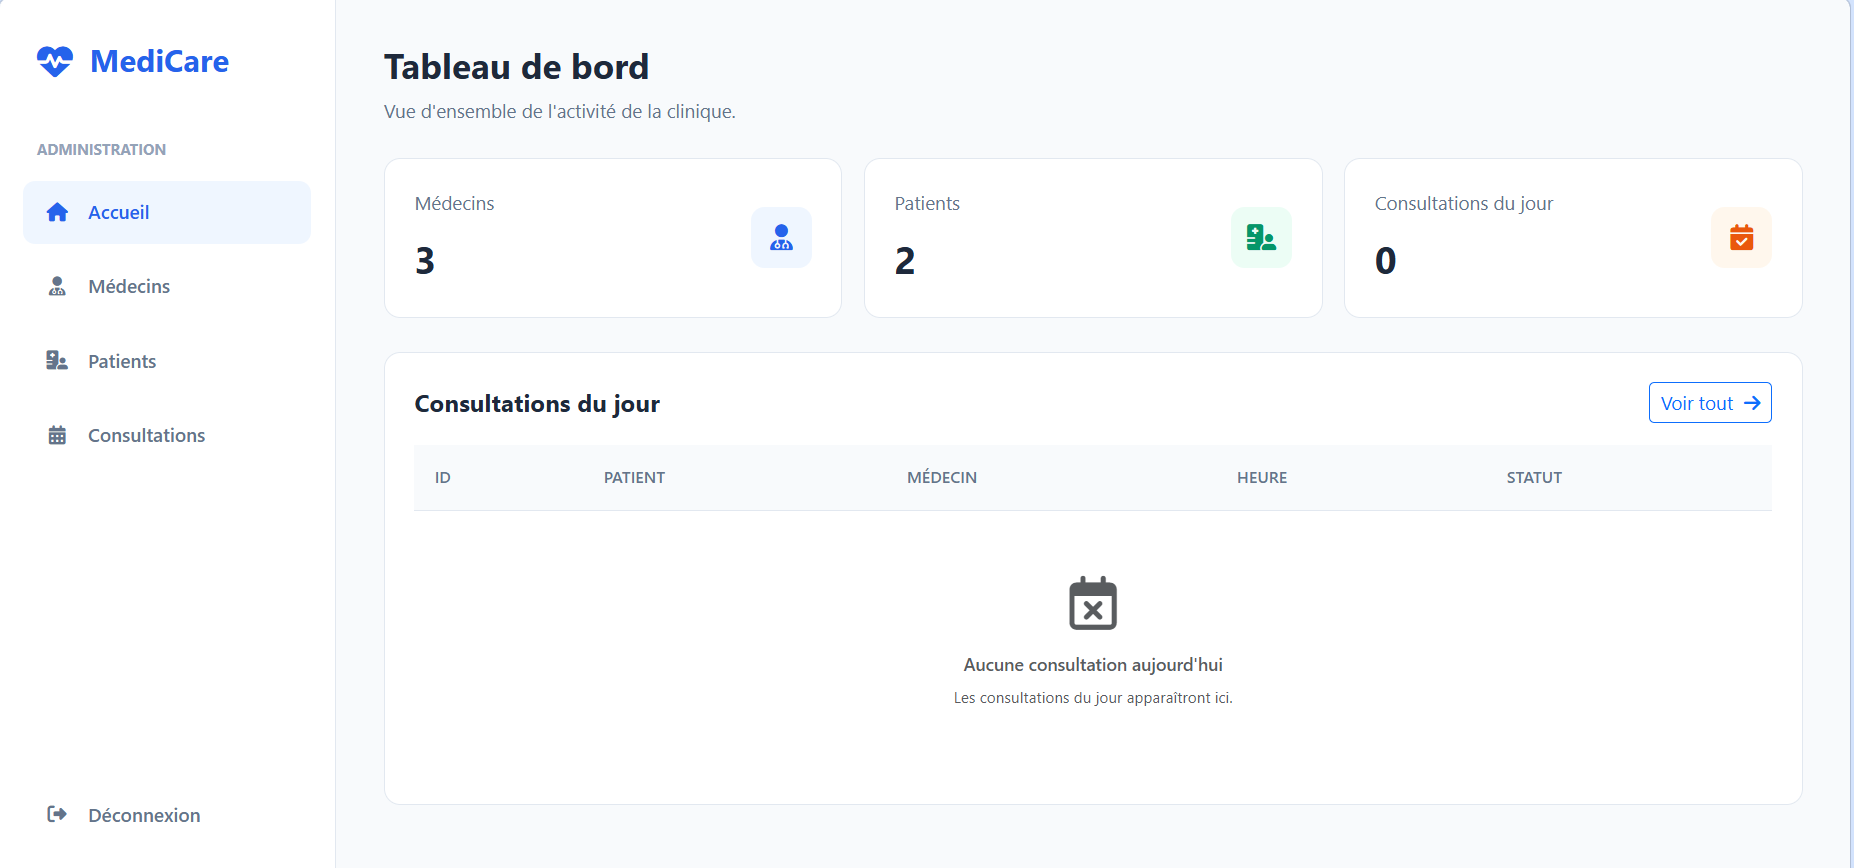
\includegraphics[width=0.4\textwidth]{images/DashboardAdmin.png}
	\caption{Présentation générale des principales informations et fonctionnalités..}
\end{figure}

\subsubsection{Gestion des patients}
\begin{figure}[h!]
	\centering
	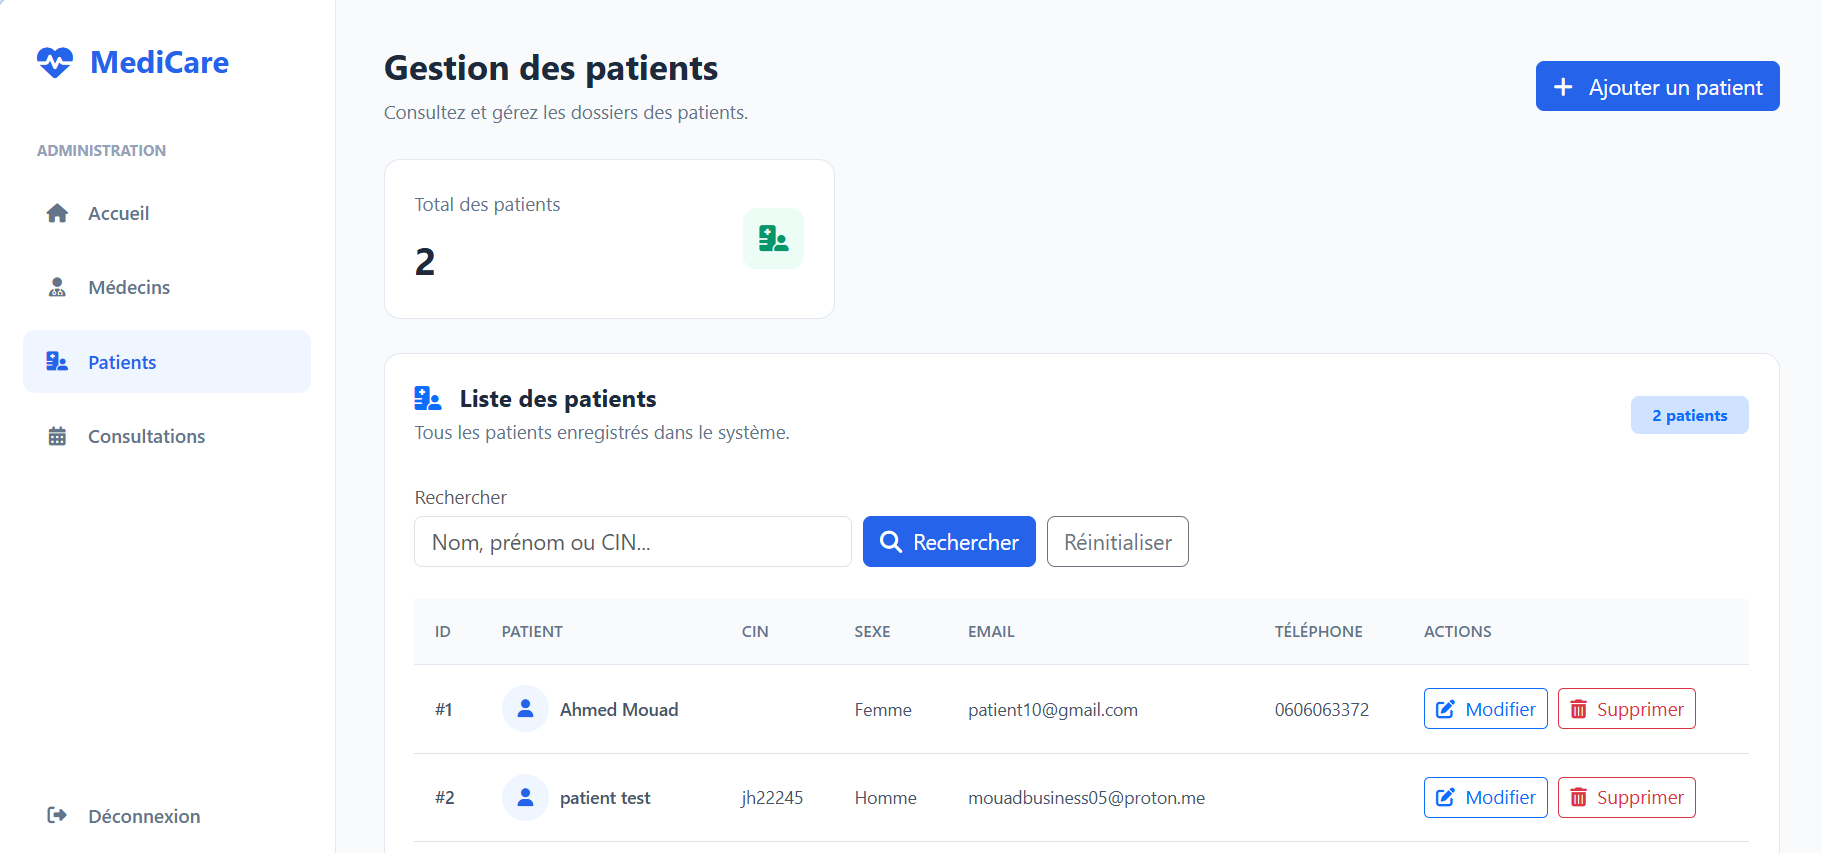
\includegraphics[width=\textwidth]{images/gestionPatients.png}
	\caption{Consultation et gestion des informations des patients .}
\end{figure}
\newpage
\subsubsection{Gestion des médecins}
\begin{figure}[h!]
	\centering
	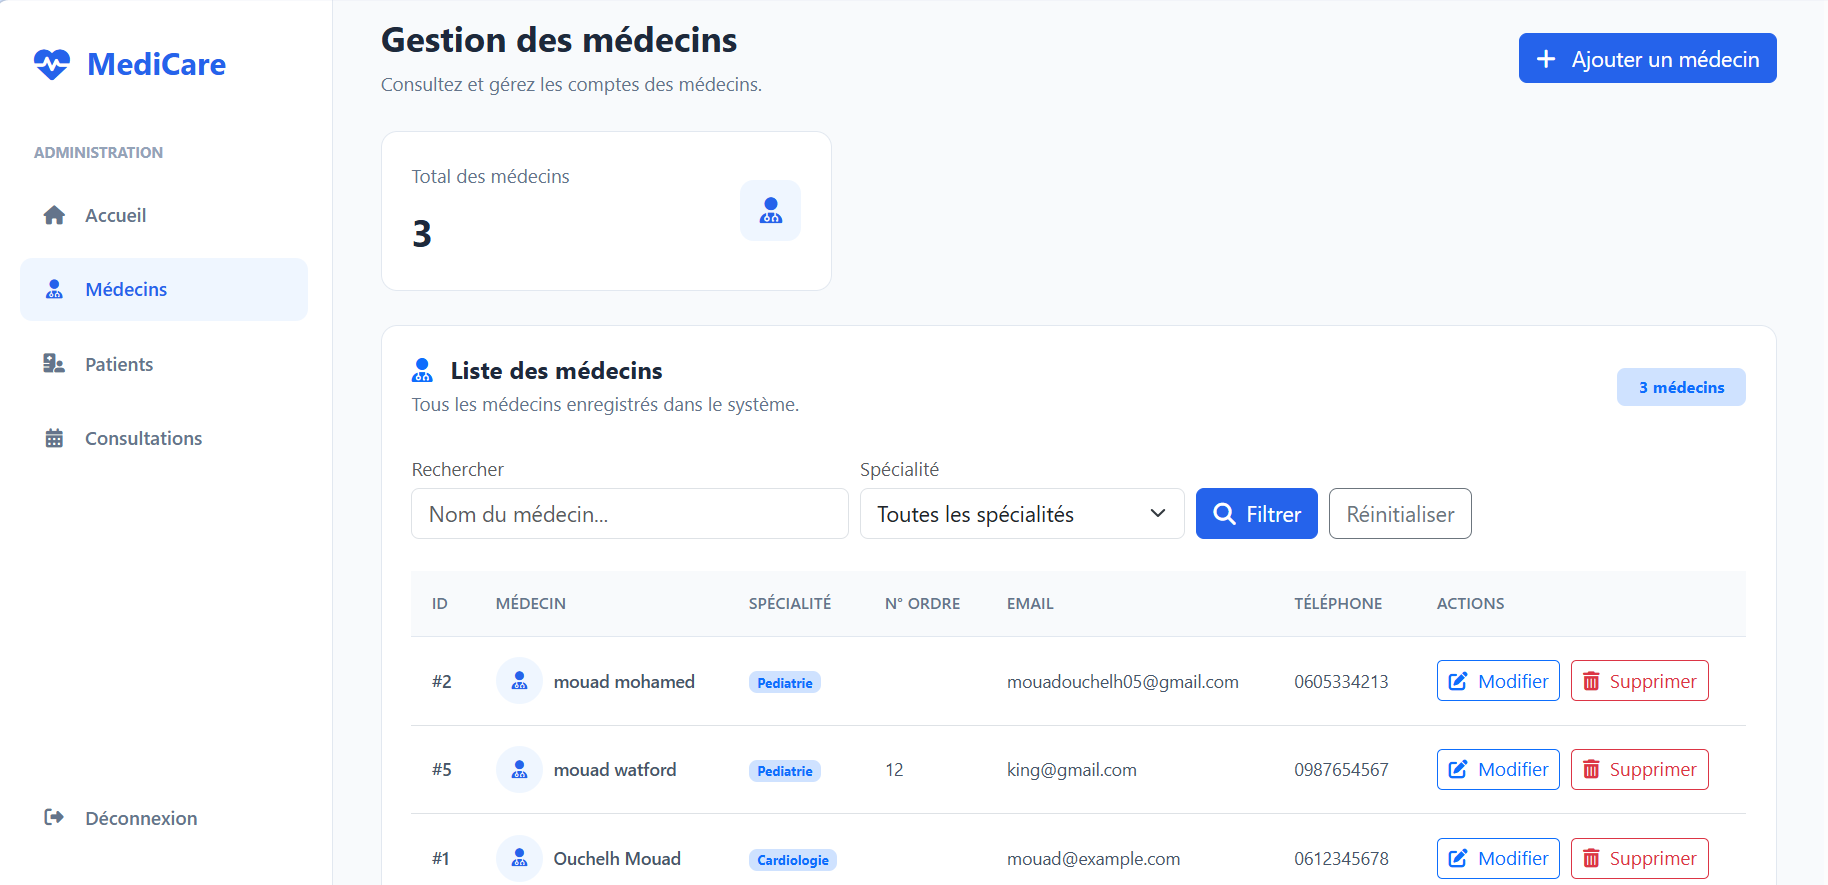
\includegraphics[width=\textwidth]{images/gestionMed.png}
	\caption{Présentation des informations relatives aux médecins.}
\end{figure}


\subsubsection{Gestion des consultations}
\begin{figure}[h!]
	\centering
	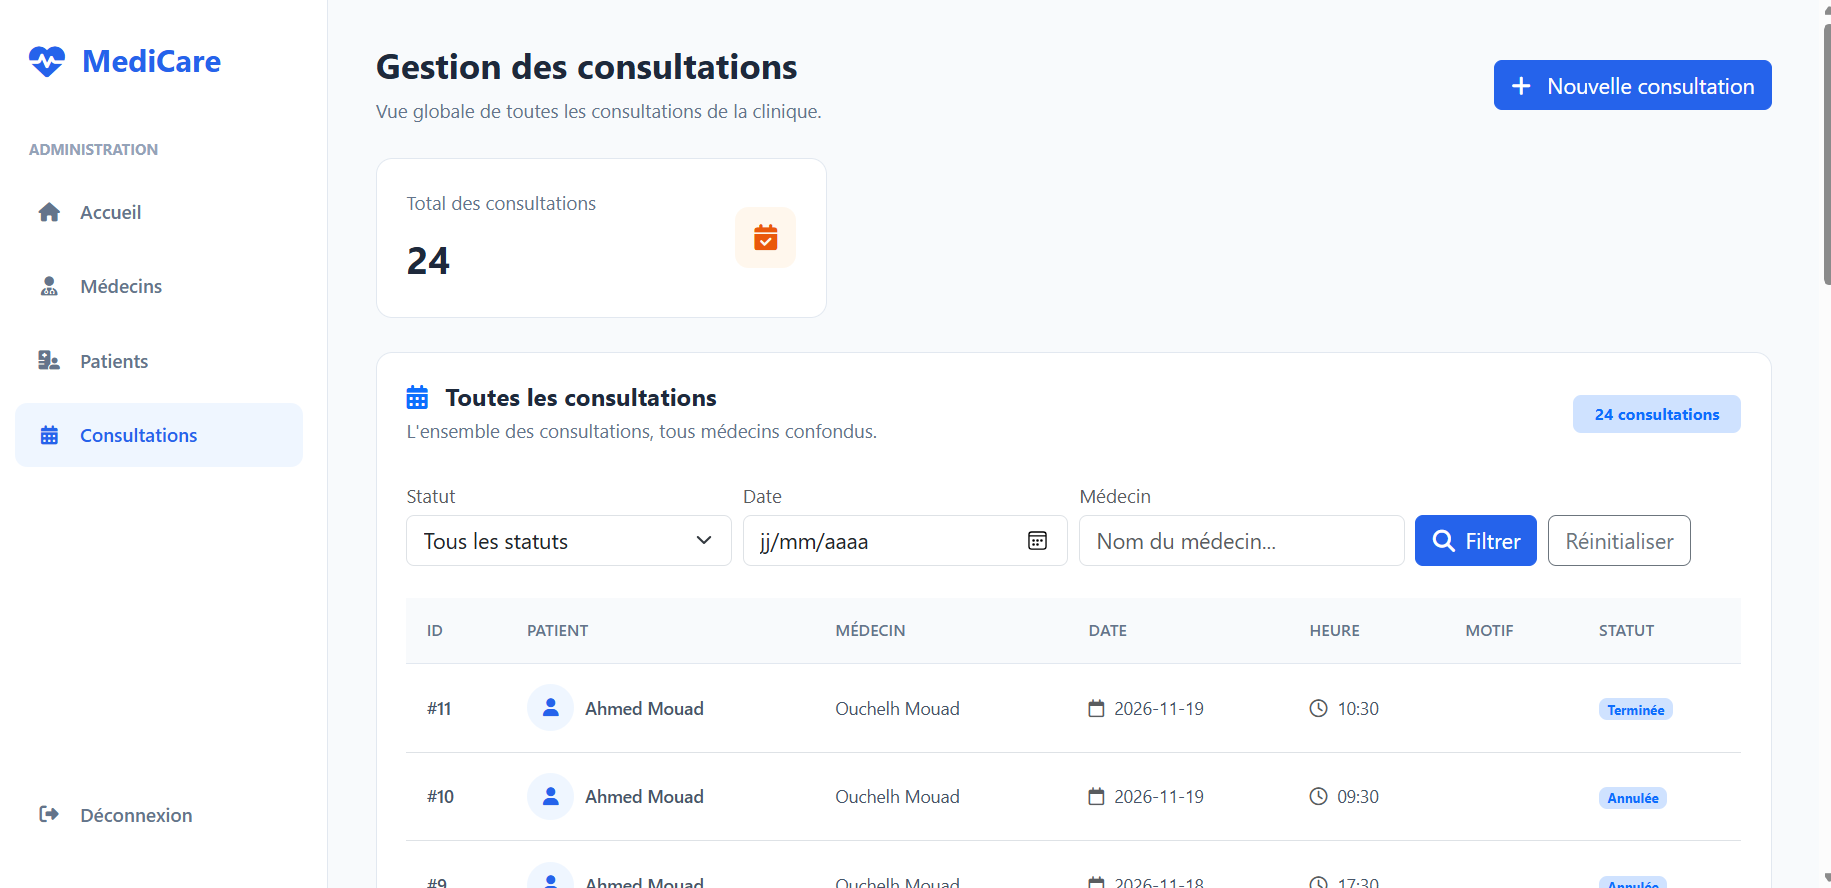
\includegraphics[width=\textwidth]{images/gestionConsultations.png}
	\caption{Interface de gestion et de suivi des consultations médicales.}
\end{figure}
